% Chapter 1

\chapter{Introducción general} % Main chapter title

\label{Chapter1} % For referencing the chapter elsewhere, use \ref{Chapter1} 
\label{IntroGeneral}

%----------------------------------------------------------------------------------------

% Define some commands to keep the formatting separated from the content 
\newcommand{\keyword}[1]{\textbf{#1}}
\newcommand{\tabhead}[1]{\textbf{#1}}
\newcommand{\code}[1]{\texttt{#1}}
\newcommand{\file}[1]{\texttt{\bfseries#1}}
\newcommand{\option}[1]{\texttt{\itshape#1}}
\newcommand{\grados}{$^{\circ}$}

%----------------------------------------------------------------------------------------
% Resumen general
En este capítulo se presenta la problemática que se buscó resolver junto con nociones sobre la tecnología LoRa y redes \emph{Mesh}.

%----------------------------------------------------------------------------------------
\section{Introducción a la tecnología LoRa}

La tecnología LoRa ha revolucionado el mundo de las comunicaciones inalámbricas al proporcionar una solución eficiente y económica para la transmisión de datos a larga distancia. Su capacidad para ofrecer una amplia cobertura y una vida útil prolongada de la batería la convierte en una opción ideal para aplicaciones de internet de las cosas y ciudades inteligentes.

En un mundo cada vez más conectado, la demanda de dispositivos y sensores interconectados ha aumentado exponencialmente. Sin embargo, muchas veces estos dispositivos necesitan transmitir datos a larga distancia sin requerir un alto consumo de energía. Ahí es donde la LoRa tiene su relevancia.

Esta tecnología de comunicación inalámbrica de largo alcance y bajo consumo de energía fue desarrollada por la empresa Semtech Corporation. \citep{WEBSITE:6} A diferencia de las redes celulares tradicionales, que priorizan la velocidad de transmisión, LoRa está diseñada específicamente para aplicaciones de IoT (\emph{Internet of Things}) que requieren una comunicación de baja velocidad y largo alcance. 

La característica más sobresaliente es su capacidad para ofrecer una cobertura excepcional. Gracias a su modulación de espectro ensanchado, puede alcanzar distancias de hasta varios kilómetros en entornos urbanos y aún más en áreas rurales. Esto hace que sea ideal para implementaciones a gran escala en ciudades inteligentes, donde se requiere una amplia cobertura para conectar sensores, medidores y otros dispositivos.

Otra ventaja importante es su eficiencia energética. Los dispositivos pueden funcionar con baterías de larga duración, incluso durante años, debido a su bajo consumo de energía. Esto resulta fundamental en aplicaciones de IoT donde los dispositivos se despliegan en lugares remotos o de difícil acceso, lo que reduce la necesidad de mantenimiento frecuente o reemplazo de baterías.

La tecnología utiliza un enfoque de comunicación denominado "comunicación de difusión". En lugar de establecer una conexión punto a punto los dispositivos, también denominados \emph{endpoints}, envían mensajes a través de múltiples saltos a través de una red gateways. Estos actúan como puntos de acceso a la infraestructura de red y retransmiten los mensajes hacia su destino final. Esto permite una arquitectura de red descentralizada y escalable, donde múltiples dispositivos pueden comunicarse simultáneamente.


Las bandas de frecuencia utilizadas son de uso compartido sin autorización, lo que significa que cualquier persona o empresa puede implementar su propia red sin tener que adquirir una licencia de espectro específica. Esto ha llevado a una rápida adopción de la tecnología en diferentes sectores, incluyendo agricultura, gestión de residuos, monitorización ambiental, logística, seguridad y más.

En resumen, la tecnología LoRa ha desempeñado un papel fundamental en el avance de la conectividad de IoT y las ciudades inteligentes. Su capacidad de ofrecer una amplia cobertura, un bajo consumo de energía y una arquitectura de red escalable la convierte en una opción atractiva para una amplia gama de aplicaciones. A medida que la tecnología continúa evolucionando, es probable que veamos aún más casos de usos innovadores y un crecimiento continuo en su adopción en todo el mundo.\citep{WEBSITE:8}


\section{Introducción a las redes Mesh}

Una red \emph{Mesh}, o red de malla, es un tipo de red de comunicación inalámbrica en la cual múltiples dispositivos se interconectan formando una estructura en forma de malla. A diferencia de las redes tradicionales en las que los dispositivos se conectan directamente a un punto central, como un enrutador, en una red \emph{Mesh} cada dispositivo actúa tanto como nodo de comunicación como de enrutador.

En una red \emph{Mesh}, todos los dispositivos se comunican entre sí de forma inalámbrica, creando una red autoorganizada y auto configurable. Cada dispositivo en la red tiene múltiples rutas para enviar y recibir datos, lo que permite una mayor resiliencia y fiabilidad en comparación con las redes tradicionales.

Cuando un dispositivo en una red \emph{Mesh} quiere enviar datos a otro dispositivo, en lugar de enviarlos directamente, los datos son enviados a través de una serie de saltos a través de otros dispositivos de la red hasta llegar al destino. Esto se logra gracias a los algoritmos de enrutamiento utilizados, los cuales determinan la mejor ruta posible para transmitir los datos basándose en factores como la calidad de la señal, la congestión de la red y la disponibilidad de los nodos.

La ventaja principal de una red \emph{Mesh} es su capacidad para extender el alcance de la red y mejorar la cobertura. Al agregar más dispositivos a la red \emph{Mesh}, se puede ampliar el área de cobertura y superar obstáculos físicos que de otro modo podrían bloquear la señal.\citep{WEBSITE:9}


\section{Estado de la solución actual}

La empresa RF Industrial, impulsora del proyecto, posee actualmente el módulo de comunicaciones “HRD-Radio-LoRa”. Haciendo uso de este es posible que un dispositivo pueda operar como un \emph{endpoint}¸ dentro de una red LoRa. Actualmente, estos módulos son utilizados en dispositivos de campo que periódicamente deben realizar el sensado de una o mas variables físicas y enviar dicha información a un servidor para su posterior procesamiento. 

Un caso de uso que presenta especial dificultad es el monitoreo de los yacimientos de petróleo. Su geografía, posición geográfica y extensión hacen que el montaje de sensores y la aplicación de tecnologías de comunicación de datos resulten un enorme desafío.
 
Otro caso de uso que puede mencionarse es el agro, en donde al igual que en los yacimientos de petróleo, las extensiones son muy grandes y en general no hay cobertura de otras redes de comunicaciones más convencionales, como puede ser la red de telefonía celular.

En la actualidad, la empresa ofrece su módulo basado en LoRa para brindar soluciones de comunicación a estas industrias. Sin embargo, por las características intrínsecas al funcionamiento y arquitectura de este tipo de redes, en donde existen uno o más \emph{gateways} que centralizan todo el tráfico y deben ser alcanzables por los dispositivos que acceden a la red,  lograr la robustez requerida en las comunicaciones puede ser muy difícil. Esto ocurre porque es preciso que los dispositivos puedan tener acceso a múltiples \emph{gateways} que deben ser desplegados en campo para lograr que, si alguno quedara fuera de servicio, la comunicación pueda continuarse por alguno de los otros. Esto representa un problema ya que como se mencionó previamente, en las zonas en donde se realizan los despliegues no hay fácil acceso a redes de comunicaciones ni energía eléctrica, que son elementos requeridos por un \emph{gateway} para poder operar y enviar los datos hacia su destino final.


\section{Motivación}

Lo que motivó la realización de este proyecto fue la búsqueda de una solución a la necesidad de brindar mayor robustez a las redes implementadas haciendo uso del “HRD-Radio-LoRa”. \citep{WEBSITE:5}

Para lograr esa mejora se decidió definir y desarrollar un protocolo que permita implementar una red \emph{Mesh} sobre los módulos “HRD-Radio-LoRa”.


%----------------------------------------------------------------------------------------
\section{Estado del Arte}

En los últimos años han aparecido numerosos estudios que buscan implementar multisalto, \emph{mesh} y protocolos de ruteo sobre redes basadas en LoRa. En su mayoría se han enmarcado en análisis teóricos ó implementaciones experimentales que brindan solución a casos muy específicos. \citep{WEBSITE:1} \citep{WEBSITE:2}\citep{WEBSITE:3}. Existen también en la actualidad algunas soluciones comerciales que incluyen \emph{hardware} y \emph{software}.\citep{WEBSITE:4} 

Este trabajo nace de la necesidad de implementar una red \emph{mesh} sobre LoRa a una placa preexistente y por esa razón se tomaron los trabajos mencionados en las referencias y algunos otros como fuente de ideas a partir de las cuáles se construyo un protocolo acorde a las necesidades del cliente y las características de la placa que se utilizó.\citep{WEBSITE:5} 



\section{Alcance y objetivos}

Los módulos de software resultantes del trabajo están orientados a permitir implementar una red \emph{Mesh} sobre la “HRD-Radio-LoRa”. Un esquema de la arquitectura propuesta puede observarse en la figura ~\ref{fig:Esquema de red}
Los componentes principales son:

\begin{itemize}
\item Módulo NR: software que es ejecutado sobre un nodo ruteador.
\item Módulo NF: software que es ejecutado sobre un nodo final.
\end{itemize}

El alcance del trabajo consiste en:

\begin{itemize}
\item Definir y especificar la lógica de funcionamiento que deberá tener la solución para permitir que un módulo ”HRD - Radio LoRa” pueda operar dentro de una red \emph{Mesh}.
\item Realizar la implementación de los módulos de software para que puedan ser ejecutados sobre la ”HRD - Radio LoRa”
\item Integración de los módulos desarrollados a la plataforma \emph{low code} que provee la empresa que es utilizado para realizar la configuración de una ”HRD - Radio LoRa”.

\end{itemize}

\begin{figure}
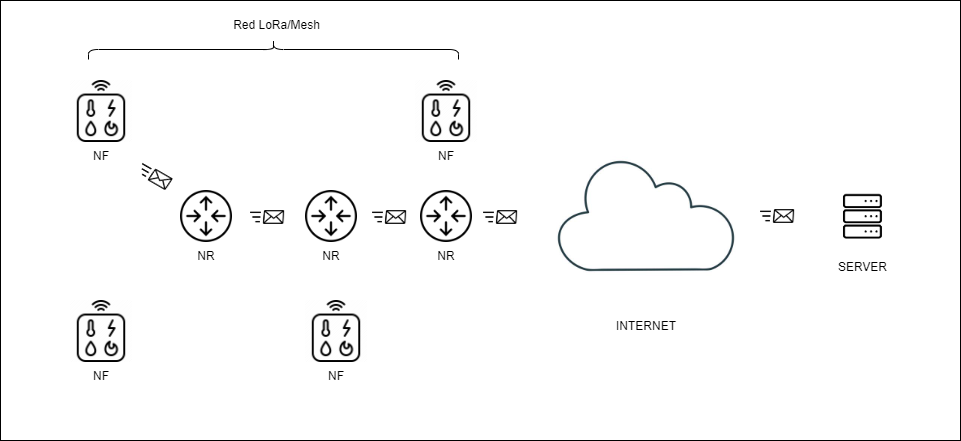
\includegraphics[width=1\textwidth]{./Figures/esquema_basico_de_red.drawio.png}
\caption{Esquema de red.}
\label{fig:Esquema de red}
\end{figure}